\section{Experimental Evaluation}
\label{sec:exp}

In order to demonstrate the efficacy of our refinement-checking approach, we
argue that our $k$-approximation:
\begin{itemize}

  \item uncovers violations with small values of $k$,

  \item can be efficiently implemented for use in systematic concurrency
  testing and long-term runtime monitoring, and
  
  \item can be efficiently implemented for use in static analysis.

\end{itemize}

To argue these points, we have studied actual C/C++ concurrent data structure
implementations, including the Scal High-Performance Multicore-Scalable
Computing suite\footnote{\url{http://scal.cs.uni-salzburg.at}}. Some of these
implementations, such as the Michael-Scott Queue~\cite{conf/podc/MichaelS96},
are meant to preserve observational refinement\footnote{More precisely, they
have been designed to be linearizable.}, while others, such as Kirsch et al.'s
$k$-FIFO~\cite{conf/pact/KirschLP13}, are meant to preserve weaker properties.
Unless otherwise noted, we use these implementations without modification,
except to annotate methods with a fixed set of possible preemption points,
e.g.,~preceding shared-memory accesses.

For our first two experiments (\S\ref{sec:exp:coverage},
\S\ref{sec:exp:dynamic}), we have developed a tool for enumerating a (possibly
large) number of alternate executions involving a limited number of object
method invocations. We run each operation on a separate thread, and execute all
thread schedules up to a given number $n \in \<Nats>$ of thread preemptions (at
specified preemption points), similarly to Microsoft's Chess
tool~\cite{conf/osdi/MusuvathiQBBNN08}. With $n=0$ preemptions, there is only
one schedule to execute, though the number of schedules grows exponentially as
$n$ increases. For instance, with our annotation of preemptions in Scal's
Michael-Scott Queue, we execute $f(n)$ schedules at a rate of roughly one
million schedules per minute, where $f$ is given by
{\footnotesize
\begin{align*}
  f(1) = 33, f(2) = 612, f(3) = 8343, f(4) = 95434, f(5) = 930141
\end{align*}}%
While similar in spirit to the second, our third experiment
(\S\ref{sec:exp:static}) executes all round-robin thread schedules up to a
given number $n \in \<Nats>$ of rounds \emph{symbolically}: we use the CSeq
tool to sequentialize a simple program which invokes a limited number of
library methods, and then CBMC (version 4.5) to perform bounded model checking
up to a given loop unroll bound. All measurements were made on similar MacBook
Pro 2.XGHz Intel Core i5/i7 machines. While space prohibits including the
entirety of our measurements, we do include a representative sample.

\subsection{Coverage of Refinement Violations}
\label{sec:exp:coverage}

To show that observational refinement violations are uncovered by our history
inclusion approximation $A_k$ for small values of $k$, we measure the number of
violations detected by a traditional linearizability checker versus those
detected by operation counting. On the one hand, the linearizability checker
detects exactly those histories $H(e)$ for which $H(e) \not\in H(L)$, due to
the equivalence of Section~\ref{sec:lin}. On the other hand, operation counting
generally provides lower fidelity: for a given $k \in \<Nats>$, one only
observes the approximation $A_k(H(e)) \preceq H(e)$, unable to resolve $H(e)$
precisely as the number of operations in $H(e)$ exceeds $k$. Thus it cannot be
the case that operation counting detects all histories which violate
observational refinement, for any fixed $k \in \<Nats>$. However, it is
theoretically possible that any given violation $H(e) \not\in H(L)$ of a
certain object could be detected by considering the approximate history
$A_k(H(e'))$ of an alternate execution $e'$ for certain $k$; that is to say
that $A_k(H(e')) \preceq H(e)$, and $A_k(H(e')) \not\in H(L)$. The interesting
empirical question is thus: for varying values of $k \in \<Nats>$, how many
violating histories $H(e)$ are ``covered'' by such an $A_k(H(e'))$?

Figure~\ref{fig:data:coverage} demonstrates that small values of $k$ suffice
for detecting violations. While $k=4$ suffices to cover all violations at
nearly all data points --- besides the first point, where the sample size of
executions is small relative to the number of operations --- all values $k > 0$
capture a nontrivial and increasing number of violations. In fact, as that
sample size increases (the x-axis is ordered by number of executions over
number of operations) the value of $k$ required to capture a violation appears
to decrease, all violations being captured by $k=3$ after a certain point. Note
that this data set only exhibits \emph{order violations} for a FIFO-based
container object, i.e.,~where elements are removed out of order; in general,
there is no cutoff value of $k \in \<Nats>$ for which all violations of such an
object can be captured; see Section~\ref{sec:containers}.

\begin{figure}
  \centering
  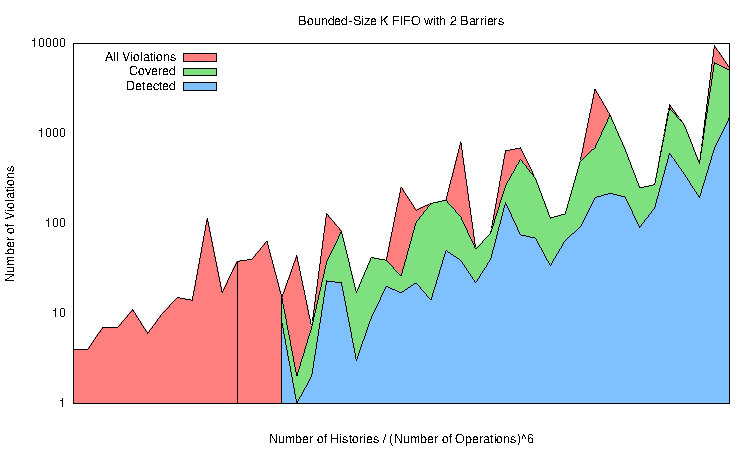
\includegraphics[width=\linewidth]{figures/coverage-bkq-2-barriers}
  \caption{Comparison of observational refinement violations detected with
    $k = 0..4$.
    Each data point measures histories on a logarithmic scale over all
    executions up to $5$ preemptions on Scal's nonblocking bounded-reordering
    queue with $i$ enqueue operations and $j$ dequeue operations.
    The x-axis is ordered by increasing number of executions over $(i+j)$,
    for $i$ and $j$ ranging over $1..4$, and only points with over $1000$
    executions are shown.
    The largest data points measure the total number of unique histories
    encountered over a given set of executions; second are the number of
    those histories which violate linearizability. Next are the number of
    those violations for which weaker histories $A_k(H(e))$ are detected
    for varying values of $k$.
  }
  \label{fig:data:coverage}
\end{figure}

\subsection{Efficacy in Testing \& Runtime Monitoring}
\label{sec:exp:dynamic}

Figure~\ref{fig:data:runtime} compares the runtime overhead of our
operation-counting instrumentation for $k=2$, versus a linearization-based
instrumentation, sampling executions with up to $20$ operations on Scal's
nonblocking Michael-Scott queue $L_\mathrm{msq}$. Since computing the set of
sequential histories $\ker H(L_\mathrm{msq})$ over $n$ operations becomes
prohibitively expensive as $n$ increases --- already surpassing a timeout of
$5$m for $n=7$ --- our measurements bypass the computation of $\ker
H(L_\mathrm{msq})$ entirely, and simply enumerate the linearizations of $H(e)$
for each execution $e$ without checking their inclusion $\ker
H(L_\mathrm{msq})$. Despite our best-effort-efficiency implementation of this
enumeration, one observes the cost incurred by this exponential-time algorithm:
as the number of operations increases --- thus exponentially increasing the
number linearizations --- performance plummets. With only 20 operations,
instrumentation overhead is nearly 100,000\%. Operation counting avoids this
dramatic overhead; though we have not optimized our implementation, we observe
that runtime overhead stays within 30\%.

\begin{figure}
  \centering
  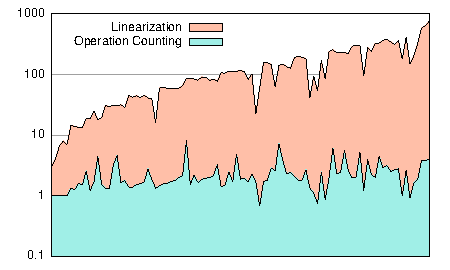
\includegraphics[width=\linewidth]{figures/lin-vs-counting-time}
  \caption{Comparison of runtime overhead between linearization-based monitoring
    and operation counting ($k=2$) for up to $20$ operations. Each data point
    measures runtime on a logarithmic scale, normalized to unmonitored
    execution time, over all executions up to $3$ preemptions on Scal's
    nonblocking Michael-Scott queue with $i$ enqueue operations and $j$ dequeue
    operations. The x-axis is ordered by increasing $i+j$, for $i$ and $j$
    ranging over $1..10$. Times do not include pre-calculation of sequential
    histories for linearization-based monitoring.
  }
  \label{fig:data:runtime}
\end{figure}

\subsection{Efficacy in Static Analysis}
\label{sec:exp:static}

We report the results of our experiments on several examples in
Table~\ref{tab:exp:static}.

\begin{table}[t]
  \footnotesize
  \begin{tabular}{llllllr}
  Example    & Bug                 & $P$ & $k$ & $m$ & $n$ & Time \\
  \hline
  %MSQueue                             & 2xEnqueue 2xDequeue & 0 & 2 & 2 & & Yes \\
  Michael-Scott & head lock      & 2x2 & 1 & 2 & 2 & 24.76s \\
  Michael-Scott & tail lock      & 3x1 & 1 & 2 & 3 & 45.44s \\
  Treiber & ABA                  & 3x4 & 1 & 1 & 2 & 52.59s \\
  Treiber & non-atomic push      & 2x2 & 1 & 1 & 2 & 24.46s \\
  Treiber & non-atomic pop       & 2x2 & 1 & 1 & 2 & 15.16s \\
  Elimination & misplaced brace  & 4x1 & 0 & 1 & 4 & 317.79s  \\
  Elimination & ``Empty''        & 3x1 & 1 & 1 & 4 & 222.04s  \\
  Elimination & ABA              & 3x4 & 0 & 1 & 2 & -- \\
  Lock-coupling & mispaced lock & 1x2 & 0 & 2 & 2 & 11.27s \\
  LFDS Queue & allocation           & 2x2 & 1 & 1 & 2 & 77.00s   
  \end{tabular} 
  \caption{Results of symbolic exploration with $A_k$ approximate refinement
    checking using CSeq \& CBMC with $m$ loop unrollings and $n$ rounds. The
    analyzed program $X$x$Y$ contains $X$ and $Y$ invocations to {\sf push} and
    {\sf pop} methods. All bugs were inserted.}
  \label{tab:exp:static}
\end{table}

TODO FIGURE OUT WHAT TO SAY HERE; PERHAPS NO NEED TO DESCRIBE ALL OF THE
STRUCTURES IN DEPTH

MSQueue (Michael \& Scott two-lock concurrent
queue~\cite{conf/podc/MichaelS96}) uses a different lock for the head and
respectively the tail of the singly-linked list used to store queue elements
(Enqueuers access only the tail while Dequeuers access only the head). We have
replaced the lock on the head (resp., tail) with a faulty lock, which enables
two concurrent Dequeues (resp, Enqueue's) to try and update the queue at the
same time, resulting in a lost update.

For the Treiber Stack, we created a version where the memory management is done
manually (using an array), in order to expose the well-known ABA bug{} to the
CBMC backend. With this change, CSeq was able to detect the ABA bug{}, using 3
{\sf push}'s, and 4 {\sf pop}'s. After fixing the ABA bug{} by removing a {\sf
free} operation, we inserted two atomicity bugs, one in the {\sf push} method,
one in the {\sf pop} method, resulting as for the MSQueue in lost updates (and
thus linearizability violations).

The Elimination Stack \citep{conf/spaa/HendlerSY04} uses the Treiber Stack as a
backend, and consequently also has the ABA bug. The Empty bug is a violation we
inserted manually, and corresponds to a {\sf pop} operation meeting a {\sf
push} operation in the collision array, but not using the value of the {\sf
push} to return. It was created by removing the line of the code where the {\sf
pop} copies the value of the corresponding {\sf push}.

The Brace bug is a violation which we originally found accidentally by making a
mistake when copying the code. Operations in the Elimination Stack first try to
access directly to the underlying Treiber Stack, then go the collision array,
and then try again to access the Treiber Stack in case nothing happened in the
collision array. In the mistake we made, a {\sf pop} operation was able to
return even in the case where this last access to the Treiber Stack fails, thus
resulting in a violation of the Stack specification.

The Lock-coupling Set also allows for a lost update violation when displacing
the {\sf unlock} commands in the code. Two {\sf remove} are able to access a
critical section at the same time, and remove the same element from the set,
resulting in a violation of the set specification.
 
In the LFDS Queue library, the user creates a queue by specifying the capacity
of the queue. We observed a violation when we create a queue whose capacity is
smaller than the number of {\sf enqueue}'s done. In our version of the code,
the actual violation is that an {\sf enqueue} is able to return successfully,
even without enqueuing anything, because of the maximum capacity of the queue
is already reached. This results in a later {\sf dequeue} returning empty, even
though an {\sf enqueue} finished successfully, which is a violation of the
Queue specification.
